% cd /storage/emulated/0/Documents/documents/latex/1920/Grade-10/2nd/circles-and-related-terms && pdflatex hand-circles-and-related-terms.tex && termux-open hand-circles-and-related-terms.pdf


\documentclass[handout]{beamer} 

\usepackage{pgfpages} 
\mode<handout>{%
\pgfpagesuselayout{4 on 1}[
%letterpaper, 
legalpaper, %landscape, 
border shrink=1mm] 
%\setbeameroption{show notes} 
}

\usepackage{xcolor}
\usepackage{anyfontsize}
\usepackage{enumitem}
\usepackage{multicol}
\usepackage{amsmath}
%\usepackage{amsfonts,dsfont}% for \mathds 
\usepackage{tabularx, booktabs, makecell} 
\usepackage{gensymb}
\usepackage{multirow}
\usepackage{graphicx, tipa}
\usepackage{tikz}
\usetikzlibrary{angles,quotes}
\usepackage{pgfplots} 
\usetikzlibrary{calc}
\pgfplotsset{compat=newest}
\usetikzlibrary{arrows.meta}
\usetikzlibrary{intersections}
\usetikzlibrary{decorations.pathreplacing}
\usepackage{flafter}
\usepackage{amsmath,amssymb,cancel,units}
\usepackage{microtype} % nicer output 
\usepackage{hfoldsty} % nicer output 
\usepackage{fixltx2e} 
\usepackage{mathptmx}
%\usepackage{mnsymbol}
\usepackage{numprint}
\usepackage[utf8]{inputenc} 
\usepackage[T1]{fontenc}

\pagenumbering{gobble}
%\linespread{0.9}
\newcommand{\vspce}{\vspace{0.75ex}}
\newcommand{\hspce}{\hspace{0.5em}}

\newcommand{\vertadjust}{\vspace*{-2.5in}} % legalpaper
%\newcommand{\vertadjust}{\vspace*{-1.5in}} % letterpaper

\newcommand{\blank}{\underline{\hspace{2em}}}%{\rule{1em}{0.15ex}}
\newcommand{\arc}[1]{{% 
\setbox9=\hbox{#1}% 
\ooalign{\resizebox{\wd9}{\height}{\texttoptiebar{\phantom{A}}}\cr#1}}}

\newcolumntype{C}{ >{\centering\arraybackslash} X}

%\frame[shrink=5] 
\begin{document} 
\vertadjust
\begin{frame} %1
\begin{center}
\textbf{Circles and Related Terms}
\end{center}

\vspace*{1ex}


\textbf{Circle: } a set of all points in a plane that are the same distance from a fixed points called the \textbf{center} 

\vspce 

\textbf{Radius:} a segment whose endpoints are the center of a circle and a point on the circle

\vspce 

\textbf{Central angle:} an angle formed by any two distinct radii of a circle

\vspce 

\textbf{Arc:} a portion of a circle that consists of two endpoints and all the points on the circle between these two endpoints

\vspce 

\begin{enumerate}[label = \alph*. ]
%A
\item \hspce \textbf{Semicircle:} an arc whose endpoints are the endpoints of a diameter
%B
\item \hspce \textbf{Minor arc:} an arc which is less than a semicircle
%C
\item \hspce \textbf{Major arc:} an arc which is more than a semicircle
\end{enumerate} 

The degree measure of a semicircle is 180\degree. 

\vspce 

The degree measure of a minor arc is the same as the degree measure ot its corresponding central angle. 

\vspce 

The degree measure of a major arc is 360\degree \hspce minus the degree measure of its corresponding minor arc. 

 
\textbf{Practice Exercises}

\vspce

A. In $\bigodot V$, $\overline{OL} $ and $\overline{CS} $ are diameters. Name the following.  
\begin{enumerate}[label = \arabic*. ]  
%%begin{multicols}{2}
%1
\item \hspce Radius 
%2
\item \hspce Central angle
%3
\item \hspce Semicircle \hspace*{4cm} %\vspace*{10cm}\hspace*{7cm}
\begin{tikzpicture}[dot/.style={circle, fill=black, inner sep=0pt, outer sep=0pt, minimum size=3pt}, dim-label/.style={fill=white, rectangle, inner sep=2pt, outer sep=0pt}, remember picture, overlay, 
nodot/.style={circle, fill=black, inner sep=0pt, outer sep=0pt, minimum size=0pt}
]  


\def\rad1{1cm}


\node(v)[dot] at (0,0) {};
\node(v-label) at ($(v)+(180:7pt)$) {$V$};

\draw[name path=circ, line width=0.5mm] (v) circle (\rad1); 

\node (a) at (0:\rad1) [nodot] {}; 
\node(a-label) at ($(a)+(0:7pt)$) {$A$};

\node (o) at (90:\rad1) [nodot]{}; 
\node(o-label) at ($(o)+(90:7pt)$) {$O$};

\node (l) at (-90:\rad1) [nodot]{}; 
\node(l-label) at ($(l)+(-90:7pt)$) {$L$}; 

\node (c) at (65:\rad1) [nodot]{}; 
\node(c-label) at ($(c)+(65:7pt)$) {$C$}; 

\node (s) at (245:\rad1) [nodot]{}; 
\node(s-label) at ($(s)+(245:7pt)$) {$S$}; 

\draw[line width=0.3mm] (o) -- (l) (c) -- (s) (a) -- (v);  

\end{tikzpicture}
%\vspace*{-3cm}\hspace*{-5cm} 
%4
\item \hspce Minor arc
%5 
\item \hspce Major arc
%\end{multicols} 
\end{enumerate}  

%%\vspace*{10cm}\hspace*{7cm}
\begin{tikzpicture}[dot/.style={circle, fill=black, inner sep=0pt, outer sep=0pt, minimum size=3pt}, dim-label/.style={fill=white, rectangle, inner sep=2pt, outer sep=0pt}, remember picture, overlay, 
nodot/.style={circle, fill=black, inner sep=0pt, outer sep=0pt, minimum size=0pt}
]  


\def\rad1{1cm}


\node(v)[dot] at (0,0) {};
\node(v-label) at ($(v)+(180:7pt)$) {$V$};

\draw[name path=circ, line width=0.5mm] (v) circle (\rad1); 

\node (a) at (0:\rad1) [nodot] {}; 
\node(a-label) at ($(a)+(0:7pt)$) {$A$};

\node (o) at (90:\rad1) [nodot]{}; 
\node(o-label) at ($(o)+(90:7pt)$) {$O$};

\node (l) at (-90:\rad1) [nodot]{}; 
\node(l-label) at ($(l)+(-90:7pt)$) {$L$}; 

\node (c) at (65:\rad1) [nodot]{}; 
\node(c-label) at ($(c)+(65:7pt)$) {$C$}; 

\node (s) at (245:\rad1) [nodot]{}; 
\node(s-label) at ($(s)+(245:7pt)$) {$S$}; 

\draw[line width=0.3mm] (o) -- (l) (c) -- (s) (a) -- (v);  

\end{tikzpicture}
%\vspace*{-3cm}\hspace*{-5cm} 
\vspace*{1.5ex}
B. In $\bigodot V$, $\overline{OL} $ and $\overline{CS} $ are diameters. If $m \angle{AVL}=90 \degree$ and $m \angle{SVL}=40 \degree$, find: 
\begin{enumerate}[label = \arabic*. ]
%begin{multicols}{3}
%1
\item \hspce m\arc{OC}
%2
\item \hspce m\arc{AL}
%3
\item \hspce m\arc{LS}
%4
\item \hspce $m \angle{CVA} $
%5
\item \hspce m\arc{CA}
%6
\item \hspce $m \angle{OVS} $
%7
\item \hspce m\arc{OS}
%8
\item \hspce m\arc{CAS}
%9
\item \hspce $m \angle{AVS} $

\end{multicols} 
\end{enumerate}  

%%\vspace*{10cm}\hspace*{7cm}
\begin{tikzpicture}[dot/.style={circle, fill=black, inner sep=0pt, outer sep=0pt, minimum size=3pt}, dim-label/.style={fill=white, rectangle, inner sep=2pt, outer sep=0pt}, remember picture, overlay, 
nodot/.style={circle, fill=black, inner sep=0pt, outer sep=0pt, minimum size=0pt}
]  


\def\rad1{1cm}


\node(v)[dot] at (0,0) {};
\node(v-label) at ($(v)+(180:7pt)$) {$V$};

\draw[name path=circ, line width=0.5mm] (v) circle (\rad1); 

\node (a) at (0:\rad1) [nodot] {}; 
\node(a-label) at ($(a)+(0:7pt)$) {$A$};

\node (o) at (90:\rad1) [nodot]{}; 
\node(o-label) at ($(o)+(90:7pt)$) {$O$};

\node (l) at (-90:\rad1) [nodot]{}; 
\node(l-label) at ($(l)+(-90:7pt)$) {$L$}; 

\node (c) at (65:\rad1) [nodot]{}; 
\node(c-label) at ($(c)+(65:7pt)$) {$C$}; 

\node (s) at (245:\rad1) [nodot]{}; 
\node(s-label) at ($(s)+(245:7pt)$) {$S$}; 

\draw[line width=0.3mm] (o) -- (l) (c) -- (s) (a) -- (v);  

\end{tikzpicture}
%\vspace*{-3cm}\hspace*{-5cm}    
\vspace*{-1.5ex}
%\textbf{Problem Set}

\vspce

A. In $\bigodot S$, $\overline{AE} $ and $\overline{MT} $ are diameters. Determine whether each arc is a minor arc, a major arc, or a semicircle. 
\begin{enumerate}[label = \arabic*. ]
%\begin{multicols*}{3}
%1
\item \hspce m\arc{MA}
%2
\item \hspce m\arc{AT}
%3
\item \hspce m\arc{ME}    
%4
\item \hspce m\arc{MET} \hspace*{5cm}%\vspace*{10cm}\hspace*{7cm}
\begin{tikzpicture}[dot/.style={circle, fill=black, inner sep=0pt, outer sep=0pt, minimum size=3pt}, 
dim-label/.style={fill=white, rectangle, inner sep=2pt, outer sep=0pt}, 
nodot/.style={circle, fill=black, inner sep=0pt, outer sep=0pt, minimum size=0pt}, 
remember picture, overlay
]  


\def\rad2{2cm}


\node(s)[dot] at (0,0) {};
\node(s-label) at ($(s)+(30:7pt)$) {$S$};

\draw[name path=circ, line width=0.5mm] (s) circle (\rad2); 

\node (t) at (-40:\rad2) [nodot] {}; 
\node(t-label) at ($(t)+(-40:7pt)$) {$T$};

\node (a) at (90:\rad2) [nodot]{}; 
\node(a-label) at ($(a)+(90:7pt)$) {$A$};

\node (e) at (-90:\rad2) [nodot]{}; 
\node(e-label) at ($(e)+(-90:7pt)$) {$E$}; 

\node (m) at (140:\rad2) [nodot]{}; 
\node(m-label) at ($(m)+(140:7pt)$) {$M$}; 

\draw[line width=0.3mm] (a) -- (e) -- (m) -- (t);  

\end{tikzpicture}
%\vspace*{-3cm}\hspace*{-5cm}
%5
\item \hspce m\arc{ET}
%6
\item \hspce m\arc{ETA}
%7
\item \hspce m\arc{MAE}
%8
\item \hspce m\arc{ATM}
%9
%\columnbreak
%\end{multicols} 
\end{enumerate}  


B. In $\bigodot S$, $\overline{AE} $ and $\overline{MT} $ are diameters and $m \angle{MSA} = 30 \degree $. Find each measure. 
\begin{enumerate}[label = \arabic*. ]
%begin{multicols}{3}
%1
\item \hspce m\arc{MA}
%2
\item \hspce m\arc{AT}
%3
\item \hspce m\arc{ME}   
%4
%5
\item \hspce m\arc{ET}
%6
%7
\item \hspce m\arc{MAE}
%8
\item \hspce m\arc{ATM}
%9

\end{multicols} 
\end{enumerate}  

 
\end{frame}

\vertadjust
\begin{frame} %2
%\begin{center}
\textbf{Circles and Related Terms}
\end{center}

\vspace*{1ex}


\textbf{Circle: } a set of all points in a plane that are the same distance from a fixed points called the \textbf{center} 

\vspce 

\textbf{Radius:} a segment whose endpoints are the center of a circle and a point on the circle

\vspce 

\textbf{Central angle:} an angle formed by any two distinct radii of a circle

\vspce 

\textbf{Arc:} a portion of a circle that consists of two endpoints and all the points on the circle between these two endpoints

\vspce 

\begin{enumerate}[label = \alph*. ]
%A
\item \hspce \textbf{Semicircle:} an arc whose endpoints are the endpoints of a diameter
%B
\item \hspce \textbf{Minor arc:} an arc which is less than a semicircle
%C
\item \hspce \textbf{Major arc:} an arc which is more than a semicircle
\end{enumerate} 

The degree measure of a semicircle is 180\degree. 

\vspce 

The degree measure of a minor arc is the same as the degree measure ot its corresponding central angle. 

\vspce 

The degree measure of a major arc is 360\degree \hspce minus the degree measure of its corresponding minor arc. 

 
%\textbf{Practice Exercises}

\vspce

A. In $\bigodot V$, $\overline{OL} $ and $\overline{CS} $ are diameters. Name the following.  
\begin{enumerate}[label = \arabic*. ]  
%%begin{multicols}{2}
%1
\item \hspce Radius 
%2
\item \hspce Central angle
%3
\item \hspce Semicircle \hspace*{4cm} %\vspace*{10cm}\hspace*{7cm}
\begin{tikzpicture}[dot/.style={circle, fill=black, inner sep=0pt, outer sep=0pt, minimum size=3pt}, dim-label/.style={fill=white, rectangle, inner sep=2pt, outer sep=0pt}, remember picture, overlay, 
nodot/.style={circle, fill=black, inner sep=0pt, outer sep=0pt, minimum size=0pt}
]  


\def\rad1{1cm}


\node(v)[dot] at (0,0) {};
\node(v-label) at ($(v)+(180:7pt)$) {$V$};

\draw[name path=circ, line width=0.5mm] (v) circle (\rad1); 

\node (a) at (0:\rad1) [nodot] {}; 
\node(a-label) at ($(a)+(0:7pt)$) {$A$};

\node (o) at (90:\rad1) [nodot]{}; 
\node(o-label) at ($(o)+(90:7pt)$) {$O$};

\node (l) at (-90:\rad1) [nodot]{}; 
\node(l-label) at ($(l)+(-90:7pt)$) {$L$}; 

\node (c) at (65:\rad1) [nodot]{}; 
\node(c-label) at ($(c)+(65:7pt)$) {$C$}; 

\node (s) at (245:\rad1) [nodot]{}; 
\node(s-label) at ($(s)+(245:7pt)$) {$S$}; 

\draw[line width=0.3mm] (o) -- (l) (c) -- (s) (a) -- (v);  

\end{tikzpicture}
%\vspace*{-3cm}\hspace*{-5cm} 
%4
\item \hspce Minor arc
%5 
\item \hspce Major arc
%\end{multicols} 
\end{enumerate}  

%%\vspace*{10cm}\hspace*{7cm}
\begin{tikzpicture}[dot/.style={circle, fill=black, inner sep=0pt, outer sep=0pt, minimum size=3pt}, dim-label/.style={fill=white, rectangle, inner sep=2pt, outer sep=0pt}, remember picture, overlay, 
nodot/.style={circle, fill=black, inner sep=0pt, outer sep=0pt, minimum size=0pt}
]  


\def\rad1{1cm}


\node(v)[dot] at (0,0) {};
\node(v-label) at ($(v)+(180:7pt)$) {$V$};

\draw[name path=circ, line width=0.5mm] (v) circle (\rad1); 

\node (a) at (0:\rad1) [nodot] {}; 
\node(a-label) at ($(a)+(0:7pt)$) {$A$};

\node (o) at (90:\rad1) [nodot]{}; 
\node(o-label) at ($(o)+(90:7pt)$) {$O$};

\node (l) at (-90:\rad1) [nodot]{}; 
\node(l-label) at ($(l)+(-90:7pt)$) {$L$}; 

\node (c) at (65:\rad1) [nodot]{}; 
\node(c-label) at ($(c)+(65:7pt)$) {$C$}; 

\node (s) at (245:\rad1) [nodot]{}; 
\node(s-label) at ($(s)+(245:7pt)$) {$S$}; 

\draw[line width=0.3mm] (o) -- (l) (c) -- (s) (a) -- (v);  

\end{tikzpicture}
%\vspace*{-3cm}\hspace*{-5cm} 
%\vspace*{1.5ex}
B. In $\bigodot V$, $\overline{OL} $ and $\overline{CS} $ are diameters. If $m \angle{AVL}=90 \degree$ and $m \angle{SVL}=40 \degree$, find: 
\begin{enumerate}[label = \arabic*. ]
%begin{multicols}{3}
%1
\item \hspce m\arc{OC}
%2
\item \hspce m\arc{AL}
%3
\item \hspce m\arc{LS}
%4
\item \hspce $m \angle{CVA} $
%5
\item \hspce m\arc{CA}
%6
\item \hspce $m \angle{OVS} $
%7
\item \hspce m\arc{OS}
%8
\item \hspce m\arc{CAS}
%9
\item \hspce $m \angle{AVS} $

\end{multicols} 
\end{enumerate}  

%%\vspace*{10cm}\hspace*{7cm}
\begin{tikzpicture}[dot/.style={circle, fill=black, inner sep=0pt, outer sep=0pt, minimum size=3pt}, dim-label/.style={fill=white, rectangle, inner sep=2pt, outer sep=0pt}, remember picture, overlay, 
nodot/.style={circle, fill=black, inner sep=0pt, outer sep=0pt, minimum size=0pt}
]  


\def\rad1{1cm}


\node(v)[dot] at (0,0) {};
\node(v-label) at ($(v)+(180:7pt)$) {$V$};

\draw[name path=circ, line width=0.5mm] (v) circle (\rad1); 

\node (a) at (0:\rad1) [nodot] {}; 
\node(a-label) at ($(a)+(0:7pt)$) {$A$};

\node (o) at (90:\rad1) [nodot]{}; 
\node(o-label) at ($(o)+(90:7pt)$) {$O$};

\node (l) at (-90:\rad1) [nodot]{}; 
\node(l-label) at ($(l)+(-90:7pt)$) {$L$}; 

\node (c) at (65:\rad1) [nodot]{}; 
\node(c-label) at ($(c)+(65:7pt)$) {$C$}; 

\node (s) at (245:\rad1) [nodot]{}; 
\node(s-label) at ($(s)+(245:7pt)$) {$S$}; 

\draw[line width=0.3mm] (o) -- (l) (c) -- (s) (a) -- (v);  

\end{tikzpicture}
%\vspace*{-3cm}\hspace*{-5cm}    
\vspace*{-1.5ex}
\textbf{Problem Set}

\vspce

A. In $\bigodot S$, $\overline{AE} $ and $\overline{MT} $ are diameters. Determine whether each arc is a minor arc, a major arc, or a semicircle. 
\begin{enumerate}[label = \arabic*. ]
%\begin{multicols*}{3}
%1
\item \hspce m\arc{MA}
%2
\item \hspce m\arc{AT}
%3
\item \hspce m\arc{ME}    
%4
\item \hspce m\arc{MET} \hspace*{5cm}%\vspace*{10cm}\hspace*{7cm}
\begin{tikzpicture}[dot/.style={circle, fill=black, inner sep=0pt, outer sep=0pt, minimum size=3pt}, 
dim-label/.style={fill=white, rectangle, inner sep=2pt, outer sep=0pt}, 
nodot/.style={circle, fill=black, inner sep=0pt, outer sep=0pt, minimum size=0pt}, 
remember picture, overlay
]  


\def\rad2{2cm}


\node(s)[dot] at (0,0) {};
\node(s-label) at ($(s)+(30:7pt)$) {$S$};

\draw[name path=circ, line width=0.5mm] (s) circle (\rad2); 

\node (t) at (-40:\rad2) [nodot] {}; 
\node(t-label) at ($(t)+(-40:7pt)$) {$T$};

\node (a) at (90:\rad2) [nodot]{}; 
\node(a-label) at ($(a)+(90:7pt)$) {$A$};

\node (e) at (-90:\rad2) [nodot]{}; 
\node(e-label) at ($(e)+(-90:7pt)$) {$E$}; 

\node (m) at (140:\rad2) [nodot]{}; 
\node(m-label) at ($(m)+(140:7pt)$) {$M$}; 

\draw[line width=0.3mm] (a) -- (e) -- (m) -- (t);  

\end{tikzpicture}
%\vspace*{-3cm}\hspace*{-5cm}
%5
\item \hspce m\arc{ET}
%6
\item \hspce m\arc{ETA}
%7
\item \hspce m\arc{MAE}
%8
\item \hspce m\arc{ATM}
%9
%\columnbreak
%\end{multicols} 
\end{enumerate}  


B. In $\bigodot S$, $\overline{AE} $ and $\overline{MT} $ are diameters and $m \angle{MSA} = 30 \degree $. Find each measure. 
\begin{enumerate}[label = \arabic*. ]
%begin{multicols}{3}
%1
\item \hspce m\arc{MA}
%2
\item \hspce m\arc{AT}
%3
\item \hspce m\arc{ME}   
%4
%5
\item \hspce m\arc{ET}
%6
%7
\item \hspce m\arc{MAE}
%8
\item \hspce m\arc{ATM}
%9

\end{multicols} 
\end{enumerate}  

 
\end{frame}

%\vspace*{-2.7in} %legalpaper
\vertadjust
\begin{frame} %3
\begin{center}
\textbf{Circles and Related Terms}
\end{center}

\vspace*{1ex}


\textbf{Circle: } a set of all points in a plane that are the same distance from a fixed points called the \textbf{center} 

\vspce 

\textbf{Radius:} a segment whose endpoints are the center of a circle and a point on the circle

\vspce 

\textbf{Central angle:} an angle formed by any two distinct radii of a circle

\vspce 

\textbf{Arc:} a portion of a circle that consists of two endpoints and all the points on the circle between these two endpoints

\vspce 

\begin{enumerate}[label = \alph*. ]
%A
\item \hspce \textbf{Semicircle:} an arc whose endpoints are the endpoints of a diameter
%B
\item \hspce \textbf{Minor arc:} an arc which is less than a semicircle
%C
\item \hspce \textbf{Major arc:} an arc which is more than a semicircle
\end{enumerate} 

The degree measure of a semicircle is 180\degree. 

\vspce 

The degree measure of a minor arc is the same as the degree measure ot its corresponding central angle. 

\vspce 

The degree measure of a major arc is 360\degree \hspce minus the degree measure of its corresponding minor arc. 

 
\textbf{Practice Exercises}

\vspce

A. In $\bigodot V$, $\overline{OL} $ and $\overline{CS} $ are diameters. Name the following.  
\begin{enumerate}[label = \arabic*. ]  
%%begin{multicols}{2}
%1
\item \hspce Radius 
%2
\item \hspce Central angle
%3
\item \hspce Semicircle \hspace*{4cm} %\vspace*{10cm}\hspace*{7cm}
\begin{tikzpicture}[dot/.style={circle, fill=black, inner sep=0pt, outer sep=0pt, minimum size=3pt}, dim-label/.style={fill=white, rectangle, inner sep=2pt, outer sep=0pt}, remember picture, overlay, 
nodot/.style={circle, fill=black, inner sep=0pt, outer sep=0pt, minimum size=0pt}
]  


\def\rad1{1cm}


\node(v)[dot] at (0,0) {};
\node(v-label) at ($(v)+(180:7pt)$) {$V$};

\draw[name path=circ, line width=0.5mm] (v) circle (\rad1); 

\node (a) at (0:\rad1) [nodot] {}; 
\node(a-label) at ($(a)+(0:7pt)$) {$A$};

\node (o) at (90:\rad1) [nodot]{}; 
\node(o-label) at ($(o)+(90:7pt)$) {$O$};

\node (l) at (-90:\rad1) [nodot]{}; 
\node(l-label) at ($(l)+(-90:7pt)$) {$L$}; 

\node (c) at (65:\rad1) [nodot]{}; 
\node(c-label) at ($(c)+(65:7pt)$) {$C$}; 

\node (s) at (245:\rad1) [nodot]{}; 
\node(s-label) at ($(s)+(245:7pt)$) {$S$}; 

\draw[line width=0.3mm] (o) -- (l) (c) -- (s) (a) -- (v);  

\end{tikzpicture}
%\vspace*{-3cm}\hspace*{-5cm} 
%4
\item \hspce Minor arc
%5 
\item \hspce Major arc
%\end{multicols} 
\end{enumerate}  

%%\vspace*{10cm}\hspace*{7cm}
\begin{tikzpicture}[dot/.style={circle, fill=black, inner sep=0pt, outer sep=0pt, minimum size=3pt}, dim-label/.style={fill=white, rectangle, inner sep=2pt, outer sep=0pt}, remember picture, overlay, 
nodot/.style={circle, fill=black, inner sep=0pt, outer sep=0pt, minimum size=0pt}
]  


\def\rad1{1cm}


\node(v)[dot] at (0,0) {};
\node(v-label) at ($(v)+(180:7pt)$) {$V$};

\draw[name path=circ, line width=0.5mm] (v) circle (\rad1); 

\node (a) at (0:\rad1) [nodot] {}; 
\node(a-label) at ($(a)+(0:7pt)$) {$A$};

\node (o) at (90:\rad1) [nodot]{}; 
\node(o-label) at ($(o)+(90:7pt)$) {$O$};

\node (l) at (-90:\rad1) [nodot]{}; 
\node(l-label) at ($(l)+(-90:7pt)$) {$L$}; 

\node (c) at (65:\rad1) [nodot]{}; 
\node(c-label) at ($(c)+(65:7pt)$) {$C$}; 

\node (s) at (245:\rad1) [nodot]{}; 
\node(s-label) at ($(s)+(245:7pt)$) {$S$}; 

\draw[line width=0.3mm] (o) -- (l) (c) -- (s) (a) -- (v);  

\end{tikzpicture}
%\vspace*{-3cm}\hspace*{-5cm} 
\vspace*{1.5ex}
B. In $\bigodot V$, $\overline{OL} $ and $\overline{CS} $ are diameters. If $m \angle{AVL}=90 \degree$ and $m \angle{SVL}=40 \degree$, find: 
\begin{enumerate}[label = \arabic*. ]
%begin{multicols}{3}
%1
\item \hspce m\arc{OC}
%2
\item \hspce m\arc{AL}
%3
\item \hspce m\arc{LS}
%4
\item \hspce $m \angle{CVA} $
%5
\item \hspce m\arc{CA}
%6
\item \hspce $m \angle{OVS} $
%7
\item \hspce m\arc{OS}
%8
\item \hspce m\arc{CAS}
%9
\item \hspce $m \angle{AVS} $

\end{multicols} 
\end{enumerate}  

%%\vspace*{10cm}\hspace*{7cm}
\begin{tikzpicture}[dot/.style={circle, fill=black, inner sep=0pt, outer sep=0pt, minimum size=3pt}, dim-label/.style={fill=white, rectangle, inner sep=2pt, outer sep=0pt}, remember picture, overlay, 
nodot/.style={circle, fill=black, inner sep=0pt, outer sep=0pt, minimum size=0pt}
]  


\def\rad1{1cm}


\node(v)[dot] at (0,0) {};
\node(v-label) at ($(v)+(180:7pt)$) {$V$};

\draw[name path=circ, line width=0.5mm] (v) circle (\rad1); 

\node (a) at (0:\rad1) [nodot] {}; 
\node(a-label) at ($(a)+(0:7pt)$) {$A$};

\node (o) at (90:\rad1) [nodot]{}; 
\node(o-label) at ($(o)+(90:7pt)$) {$O$};

\node (l) at (-90:\rad1) [nodot]{}; 
\node(l-label) at ($(l)+(-90:7pt)$) {$L$}; 

\node (c) at (65:\rad1) [nodot]{}; 
\node(c-label) at ($(c)+(65:7pt)$) {$C$}; 

\node (s) at (245:\rad1) [nodot]{}; 
\node(s-label) at ($(s)+(245:7pt)$) {$S$}; 

\draw[line width=0.3mm] (o) -- (l) (c) -- (s) (a) -- (v);  

\end{tikzpicture}
%\vspace*{-3cm}\hspace*{-5cm}    
\vspace*{-1.5ex}
%\textbf{Problem Set}

\vspce

A. In $\bigodot S$, $\overline{AE} $ and $\overline{MT} $ are diameters. Determine whether each arc is a minor arc, a major arc, or a semicircle. 
\begin{enumerate}[label = \arabic*. ]
%\begin{multicols*}{3}
%1
\item \hspce m\arc{MA}
%2
\item \hspce m\arc{AT}
%3
\item \hspce m\arc{ME}    
%4
\item \hspce m\arc{MET} \hspace*{5cm}%\vspace*{10cm}\hspace*{7cm}
\begin{tikzpicture}[dot/.style={circle, fill=black, inner sep=0pt, outer sep=0pt, minimum size=3pt}, 
dim-label/.style={fill=white, rectangle, inner sep=2pt, outer sep=0pt}, 
nodot/.style={circle, fill=black, inner sep=0pt, outer sep=0pt, minimum size=0pt}, 
remember picture, overlay
]  


\def\rad2{2cm}


\node(s)[dot] at (0,0) {};
\node(s-label) at ($(s)+(30:7pt)$) {$S$};

\draw[name path=circ, line width=0.5mm] (s) circle (\rad2); 

\node (t) at (-40:\rad2) [nodot] {}; 
\node(t-label) at ($(t)+(-40:7pt)$) {$T$};

\node (a) at (90:\rad2) [nodot]{}; 
\node(a-label) at ($(a)+(90:7pt)$) {$A$};

\node (e) at (-90:\rad2) [nodot]{}; 
\node(e-label) at ($(e)+(-90:7pt)$) {$E$}; 

\node (m) at (140:\rad2) [nodot]{}; 
\node(m-label) at ($(m)+(140:7pt)$) {$M$}; 

\draw[line width=0.3mm] (a) -- (e) -- (m) -- (t);  

\end{tikzpicture}
%\vspace*{-3cm}\hspace*{-5cm}
%5
\item \hspce m\arc{ET}
%6
\item \hspce m\arc{ETA}
%7
\item \hspce m\arc{MAE}
%8
\item \hspce m\arc{ATM}
%9
%\columnbreak
%\end{multicols} 
\end{enumerate}  


B. In $\bigodot S$, $\overline{AE} $ and $\overline{MT} $ are diameters and $m \angle{MSA} = 30 \degree $. Find each measure. 
\begin{enumerate}[label = \arabic*. ]
%begin{multicols}{3}
%1
\item \hspce m\arc{MA}
%2
\item \hspce m\arc{AT}
%3
\item \hspce m\arc{ME}   
%4
%5
\item \hspce m\arc{ET}
%6
%7
\item \hspce m\arc{MAE}
%8
\item \hspce m\arc{ATM}
%9

\end{multicols} 
\end{enumerate}  

 
\end{frame}

%\vspace*{-2.7in} %legalpaper
\vertadjust
\begin{frame} %4
%\begin{center}
\textbf{Circles and Related Terms}
\end{center}

\vspace*{1ex}


\textbf{Circle: } a set of all points in a plane that are the same distance from a fixed points called the \textbf{center} 

\vspce 

\textbf{Radius:} a segment whose endpoints are the center of a circle and a point on the circle

\vspce 

\textbf{Central angle:} an angle formed by any two distinct radii of a circle

\vspce 

\textbf{Arc:} a portion of a circle that consists of two endpoints and all the points on the circle between these two endpoints

\vspce 

\begin{enumerate}[label = \alph*. ]
%A
\item \hspce \textbf{Semicircle:} an arc whose endpoints are the endpoints of a diameter
%B
\item \hspce \textbf{Minor arc:} an arc which is less than a semicircle
%C
\item \hspce \textbf{Major arc:} an arc which is more than a semicircle
\end{enumerate} 

The degree measure of a semicircle is 180\degree. 

\vspce 

The degree measure of a minor arc is the same as the degree measure ot its corresponding central angle. 

\vspce 

The degree measure of a major arc is 360\degree \hspce minus the degree measure of its corresponding minor arc. 

 
%\textbf{Practice Exercises}

\vspce

A. In $\bigodot V$, $\overline{OL} $ and $\overline{CS} $ are diameters. Name the following.  
\begin{enumerate}[label = \arabic*. ]  
%%begin{multicols}{2}
%1
\item \hspce Radius 
%2
\item \hspce Central angle
%3
\item \hspce Semicircle \hspace*{4cm} %\vspace*{10cm}\hspace*{7cm}
\begin{tikzpicture}[dot/.style={circle, fill=black, inner sep=0pt, outer sep=0pt, minimum size=3pt}, dim-label/.style={fill=white, rectangle, inner sep=2pt, outer sep=0pt}, remember picture, overlay, 
nodot/.style={circle, fill=black, inner sep=0pt, outer sep=0pt, minimum size=0pt}
]  


\def\rad1{1cm}


\node(v)[dot] at (0,0) {};
\node(v-label) at ($(v)+(180:7pt)$) {$V$};

\draw[name path=circ, line width=0.5mm] (v) circle (\rad1); 

\node (a) at (0:\rad1) [nodot] {}; 
\node(a-label) at ($(a)+(0:7pt)$) {$A$};

\node (o) at (90:\rad1) [nodot]{}; 
\node(o-label) at ($(o)+(90:7pt)$) {$O$};

\node (l) at (-90:\rad1) [nodot]{}; 
\node(l-label) at ($(l)+(-90:7pt)$) {$L$}; 

\node (c) at (65:\rad1) [nodot]{}; 
\node(c-label) at ($(c)+(65:7pt)$) {$C$}; 

\node (s) at (245:\rad1) [nodot]{}; 
\node(s-label) at ($(s)+(245:7pt)$) {$S$}; 

\draw[line width=0.3mm] (o) -- (l) (c) -- (s) (a) -- (v);  

\end{tikzpicture}
%\vspace*{-3cm}\hspace*{-5cm} 
%4
\item \hspce Minor arc
%5 
\item \hspce Major arc
%\end{multicols} 
\end{enumerate}  

%%\vspace*{10cm}\hspace*{7cm}
\begin{tikzpicture}[dot/.style={circle, fill=black, inner sep=0pt, outer sep=0pt, minimum size=3pt}, dim-label/.style={fill=white, rectangle, inner sep=2pt, outer sep=0pt}, remember picture, overlay, 
nodot/.style={circle, fill=black, inner sep=0pt, outer sep=0pt, minimum size=0pt}
]  


\def\rad1{1cm}


\node(v)[dot] at (0,0) {};
\node(v-label) at ($(v)+(180:7pt)$) {$V$};

\draw[name path=circ, line width=0.5mm] (v) circle (\rad1); 

\node (a) at (0:\rad1) [nodot] {}; 
\node(a-label) at ($(a)+(0:7pt)$) {$A$};

\node (o) at (90:\rad1) [nodot]{}; 
\node(o-label) at ($(o)+(90:7pt)$) {$O$};

\node (l) at (-90:\rad1) [nodot]{}; 
\node(l-label) at ($(l)+(-90:7pt)$) {$L$}; 

\node (c) at (65:\rad1) [nodot]{}; 
\node(c-label) at ($(c)+(65:7pt)$) {$C$}; 

\node (s) at (245:\rad1) [nodot]{}; 
\node(s-label) at ($(s)+(245:7pt)$) {$S$}; 

\draw[line width=0.3mm] (o) -- (l) (c) -- (s) (a) -- (v);  

\end{tikzpicture}
%\vspace*{-3cm}\hspace*{-5cm} 
%\vspace*{1.5ex}
B. In $\bigodot V$, $\overline{OL} $ and $\overline{CS} $ are diameters. If $m \angle{AVL}=90 \degree$ and $m \angle{SVL}=40 \degree$, find: 
\begin{enumerate}[label = \arabic*. ]
%begin{multicols}{3}
%1
\item \hspce m\arc{OC}
%2
\item \hspce m\arc{AL}
%3
\item \hspce m\arc{LS}
%4
\item \hspce $m \angle{CVA} $
%5
\item \hspce m\arc{CA}
%6
\item \hspce $m \angle{OVS} $
%7
\item \hspce m\arc{OS}
%8
\item \hspce m\arc{CAS}
%9
\item \hspce $m \angle{AVS} $

\end{multicols} 
\end{enumerate}  

%%\vspace*{10cm}\hspace*{7cm}
\begin{tikzpicture}[dot/.style={circle, fill=black, inner sep=0pt, outer sep=0pt, minimum size=3pt}, dim-label/.style={fill=white, rectangle, inner sep=2pt, outer sep=0pt}, remember picture, overlay, 
nodot/.style={circle, fill=black, inner sep=0pt, outer sep=0pt, minimum size=0pt}
]  


\def\rad1{1cm}


\node(v)[dot] at (0,0) {};
\node(v-label) at ($(v)+(180:7pt)$) {$V$};

\draw[name path=circ, line width=0.5mm] (v) circle (\rad1); 

\node (a) at (0:\rad1) [nodot] {}; 
\node(a-label) at ($(a)+(0:7pt)$) {$A$};

\node (o) at (90:\rad1) [nodot]{}; 
\node(o-label) at ($(o)+(90:7pt)$) {$O$};

\node (l) at (-90:\rad1) [nodot]{}; 
\node(l-label) at ($(l)+(-90:7pt)$) {$L$}; 

\node (c) at (65:\rad1) [nodot]{}; 
\node(c-label) at ($(c)+(65:7pt)$) {$C$}; 

\node (s) at (245:\rad1) [nodot]{}; 
\node(s-label) at ($(s)+(245:7pt)$) {$S$}; 

\draw[line width=0.3mm] (o) -- (l) (c) -- (s) (a) -- (v);  

\end{tikzpicture}
%\vspace*{-3cm}\hspace*{-5cm}    
\vspace*{-1.5ex}
\textbf{Problem Set}

\vspce

A. In $\bigodot S$, $\overline{AE} $ and $\overline{MT} $ are diameters. Determine whether each arc is a minor arc, a major arc, or a semicircle. 
\begin{enumerate}[label = \arabic*. ]
%\begin{multicols*}{3}
%1
\item \hspce m\arc{MA}
%2
\item \hspce m\arc{AT}
%3
\item \hspce m\arc{ME}    
%4
\item \hspce m\arc{MET} \hspace*{5cm}%\vspace*{10cm}\hspace*{7cm}
\begin{tikzpicture}[dot/.style={circle, fill=black, inner sep=0pt, outer sep=0pt, minimum size=3pt}, 
dim-label/.style={fill=white, rectangle, inner sep=2pt, outer sep=0pt}, 
nodot/.style={circle, fill=black, inner sep=0pt, outer sep=0pt, minimum size=0pt}, 
remember picture, overlay
]  


\def\rad2{2cm}


\node(s)[dot] at (0,0) {};
\node(s-label) at ($(s)+(30:7pt)$) {$S$};

\draw[name path=circ, line width=0.5mm] (s) circle (\rad2); 

\node (t) at (-40:\rad2) [nodot] {}; 
\node(t-label) at ($(t)+(-40:7pt)$) {$T$};

\node (a) at (90:\rad2) [nodot]{}; 
\node(a-label) at ($(a)+(90:7pt)$) {$A$};

\node (e) at (-90:\rad2) [nodot]{}; 
\node(e-label) at ($(e)+(-90:7pt)$) {$E$}; 

\node (m) at (140:\rad2) [nodot]{}; 
\node(m-label) at ($(m)+(140:7pt)$) {$M$}; 

\draw[line width=0.3mm] (a) -- (e) -- (m) -- (t);  

\end{tikzpicture}
%\vspace*{-3cm}\hspace*{-5cm}
%5
\item \hspce m\arc{ET}
%6
\item \hspce m\arc{ETA}
%7
\item \hspce m\arc{MAE}
%8
\item \hspce m\arc{ATM}
%9
%\columnbreak
%\end{multicols} 
\end{enumerate}  


B. In $\bigodot S$, $\overline{AE} $ and $\overline{MT} $ are diameters and $m \angle{MSA} = 30 \degree $. Find each measure. 
\begin{enumerate}[label = \arabic*. ]
%begin{multicols}{3}
%1
\item \hspce m\arc{MA}
%2
\item \hspce m\arc{AT}
%3
\item \hspce m\arc{ME}   
%4
%5
\item \hspce m\arc{ET}
%6
%7
\item \hspce m\arc{MAE}
%8
\item \hspce m\arc{ATM}
%9

\end{multicols} 
\end{enumerate}  

 
\end{frame}

\end{document}

